\section{相关工作}
\label{sec:related}

\noindent\textbf{表格基础模型的上下文敏感性。}
表格基础模型通过以带标签样本行为条件，对无标签查询样本进行预测。TabPFN 奠定了基于合成先验的推理范式，TabICL 将表格上下文学习扩展到更大规模的数据集，TabDPT 则将检索机制与真实数据预训练相结合~\citep{muller2023tabpfn,qu2025tabicl,ma2025tabdpt}。后续工作进一步扩展了预训练规模、可扩展性与任务覆盖范围~\citep{hollmann2025tabpfn,grinsztajn2025tabpfn25,qu2026tabiclv2}。有关上下文采样的研究还表明，上下文的规模、覆盖范围与采样方式都会影响预测准确性和稳定性~\citep{abdullah2026contextsampling}。这些工作改进了模型设计和规模，但并未在冻结模型下对不同构造方式产生的上下文预测进行组合。

\medskip
\noindent\textbf{上下文压缩、检索与选择。}
TuneTables、LoCalPFN、MixturePFN 和 Tab-AICL 分别通过压缩、检索、路由或主动获取来构造推理上下文~\citep{feuer2024tunetables,thomas2024localpfn,xu2025mixturepfn,
treerath2026tabaicl}。\method{} 将上下文选择扩展为上下文集成：上述方法通常优化或选择一个主导上下文或专家，以提高可扩展性或查询相关性；而 \method{} 则整合由异质上下文构造器诱导的预测。

\medskip
\noindent\textbf{上下文集成与构造多样性。}
在表格学习之外，已有上下文集成方法会组合由不同示例子集得到的预测；例如，DENSE 对这些预测进行平均~\citep{khalifa2023dense}。在表格预测中，TabPFN 会集成不同预处理方式以及特征或标签置换得到的变体~\citep{hollmann2025tabpfn}。\method{} 将上下文集成从同一构造方案的多个变体扩展到具有不同归纳偏置的异质构造器，并依据查询级证据分配其影响。

\begin{figure}[!t]
  \centering
  \ifdefined\ICLRLayout
    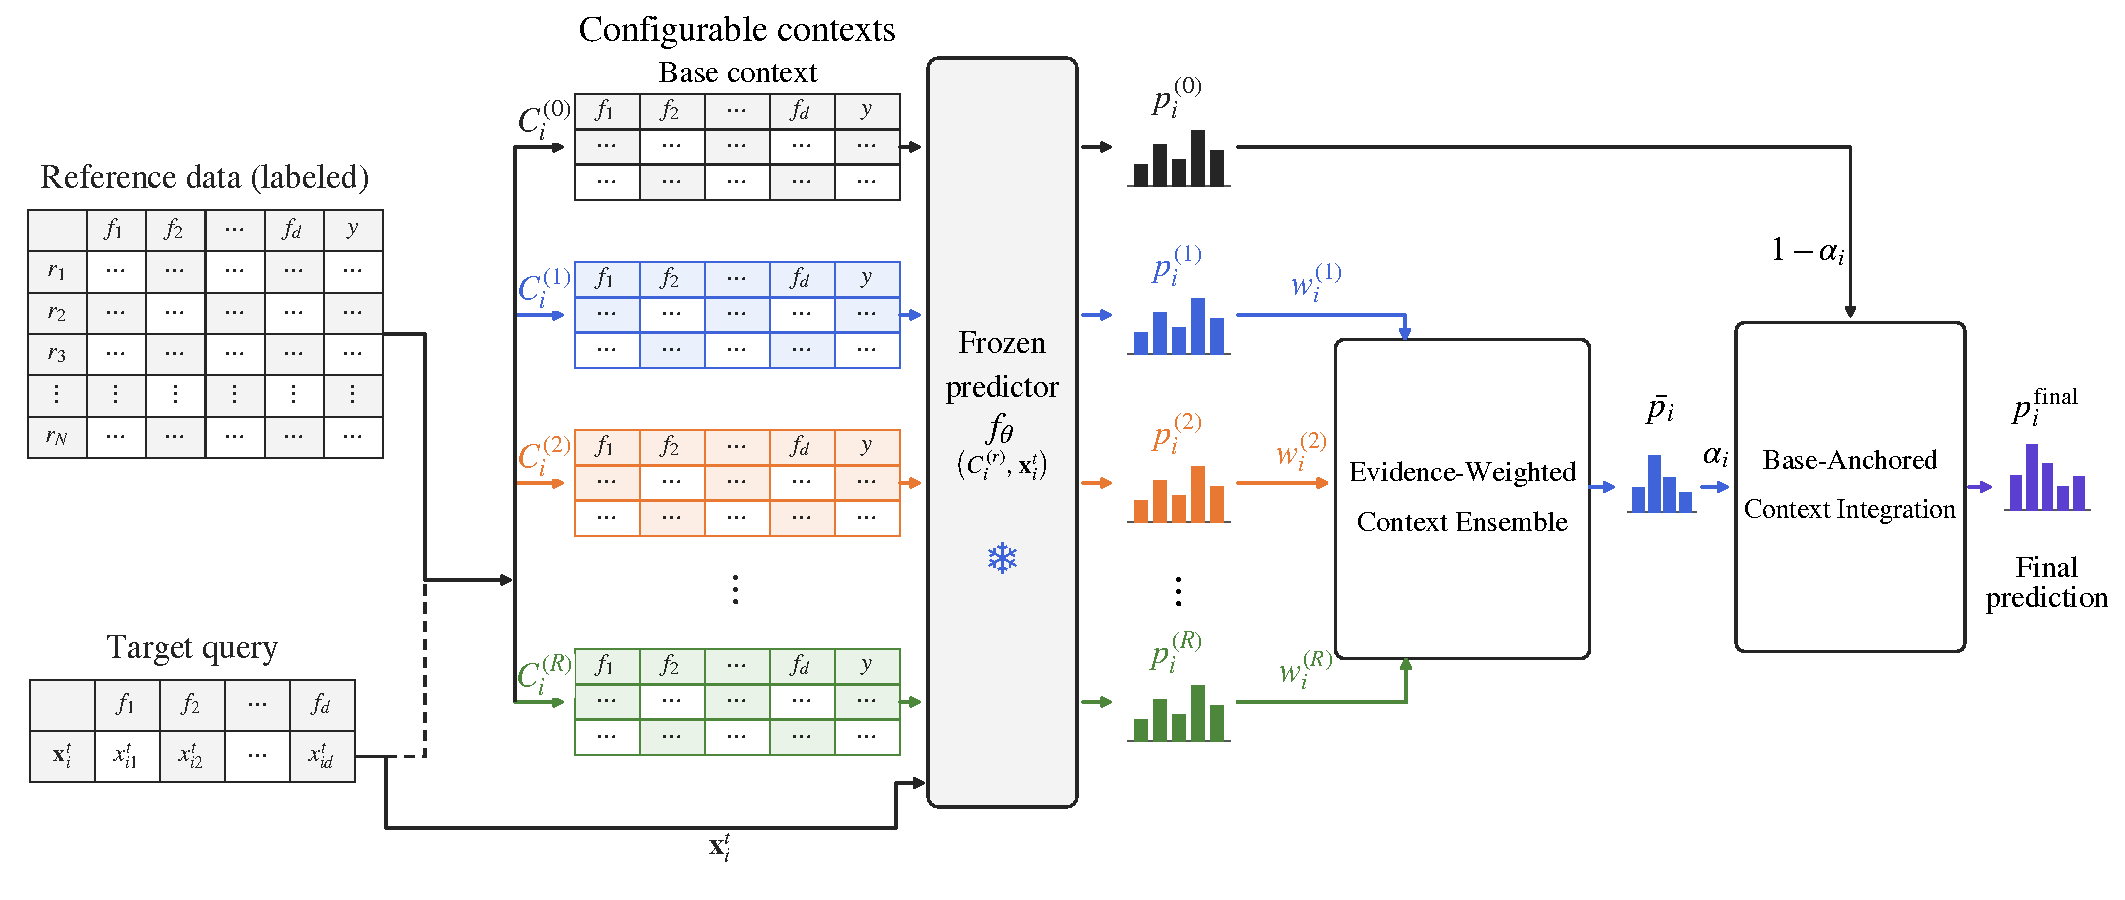
\includegraphics[width=\textwidth]{figures/context_ensemble_framework_pfn_input_semantics_fixed_lines.pdf}
  \else
    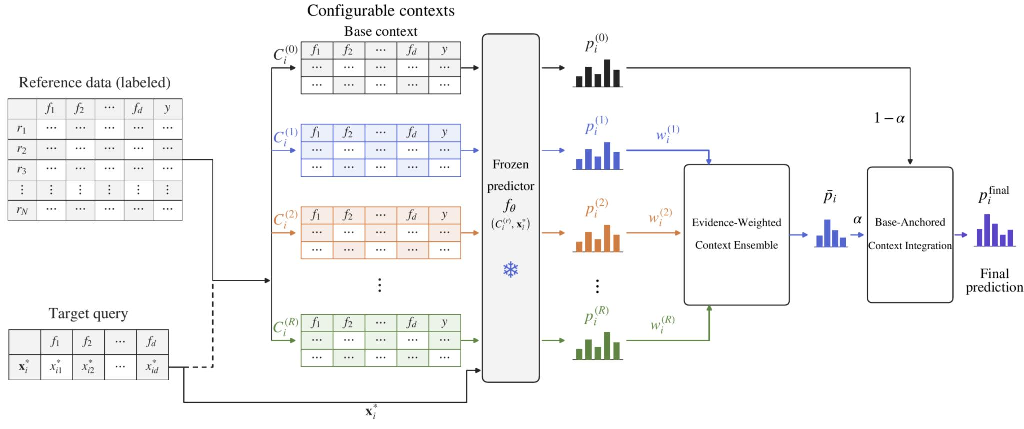
\includegraphics[width=0.86\textwidth]{figures/adaptive_context_ensemble_framework.pdf}
  \fi
  \caption{\textbf{\method{} 的框架概览。}
  对每个查询样本，冻结预测器分别评估 Base 与可配置构造器产生的替代上下文。置信度和一致性决定各替代预测的权重，查询相关门控再将其聚合结果与 Base 融合。图中的 $p_i^{(r)}$ 表示分类概率向量；回归任务在同一流程中使用标量预测 $\hat y_i^{(r)}$。}
  \label{fig:tabace_overview}
\end{figure}

\medskip
\noindent\textbf{常规条件与偏移条件下的上下文变化。}
已有研究在多种数据变化条件下考察了表格预测的稳健性。经典标签偏移方法估计或重新校准目标类别先验~\citep{lipton2018bbse,alexandari2020labelshift}；DistPFN、Drift-Resilient TabPFN 和 SPN 则分别处理表格上下文学习中的标签偏移、时间偏移与策略性偏移~\citep{lee2026distpfn,helli2024drifttabpfn,
lv2026strategic}。SkillTFM 通过按证据检索外部修复技能来适配冻结的 TFM；其运行时证书决定是否采用修复，否则回退到基础预测器~\citep{he2026skilltfm}。TableShift 与 TabFSBench 分别提供分布偏移表格任务和受控特征变化的基准~\citep{gardner2023tableshift,
cheng2025tabfsbench}。上下文采样研究还表明，即便在常规评估条件下，上下文选择也会影响 TFM 预测~\citep{abdullah2026contextsampling}。因此，我们同时在常规变化与多种受控变化类别下研究上下文聚合。
